% 5. Model Development
%   5.1. Anatomical Model
%     5.1.1. CT Image Processing: Lung Segmentation, Centreline and Radii Extraction
%     5.1.2. Algorithmic Generation of the Distal Airway Centreline
%   5.2. Mechanical Model
%     5.2.1. Programming Language --- Model Designing & Instantiating
%     5.2.1.1  Callbacks' Role in State Variables Discontinuity Handling
%     5.2.3. Model Testing

\section{Model Development}
\label{sec:model_development}

% Mettere enfasi sulla ricerca dei metodi perché Julia e non altro.

% Visione d'insieme (diagramma con flusso dell'informazione, data
% pipeline). Questo diagramma mostra a partire dagli input che ho
% avuto (TC) tutto l'iter del dato.

% Qui ha detto poi Chiara che conviene inserire delle informazioni
% riguardanti i modelli matematici utilizzati.

This chapter describes the methods used to develop an open-source, 3D
morphometric neonatal lung model that allows simulations of lung
aeration at birth.

An anatomically coherent 3D lung model is combined with a mechanical
model of the airways and acini, able to simulate changes in the
mechanical properties of the airways when the lung fluid is replaced
by air entering the lungs.

The sequence for model development is reported in
\cref{fig:data_pipeline}. We extracted a 3D surface mesh of lung lobes
and airway centrelines from a lung CT of a newborn. We implemented a
statistical method, previously described for adult lung models, able
to generate distal airways that were not visible on the CT. We adapted
the method for the newborn lung.

We implemented a mechanical model of the airways and acini whose
parameters are dependent on the airway's lengths and diameters and the
presence of fetal fluid, fetal fluid-air interface, or air in the
airway. We exploited an open-source solver for differential equations
to simulate the network.

\begin{figure}[H]\centering
  % todo: modificare l'immagine sopra ad "anatomical surrogate generation" con uno screen di ParaView.
% todo: aggiungere immagini sopra al branch del modello meccanico.

\begin{figure}[H]\centering
  \begin{tikzpicture}[node distance=3cm]
    % Nodes
    %% Chaste & Morphometric Model
    \node (ct_acquisition)           [startstop] {CT\\Acquisition};
    \node (img_ct_acquisition)       [image, above of=ct_acquisition, yshift=-1.0cm]                   {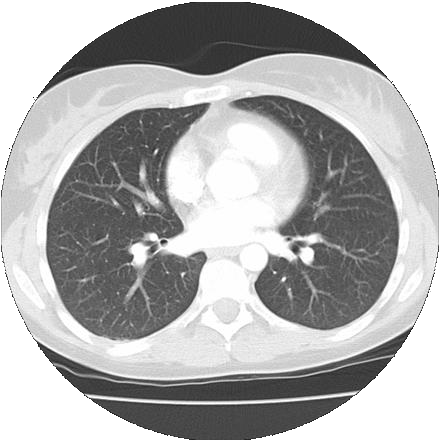
\includegraphics[width=2.0cm]{ct_acquisition.png}};
    %%% Upper branch
    \node (lobes_segmentation)       [process, right of=ct_acquisition, xshift=3.25cm, yshift=+2cm]    {Lobes\\segmentation};
    %%% Lower branch
    \node (img_lobes_segmentation)   [image, above of=lobes_segmentation, xshift=-.1cm, yshift=-1.2cm] {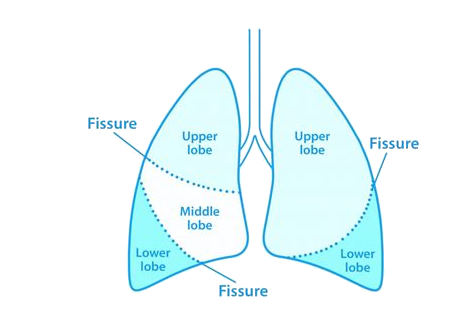
\includegraphics[width=3.5cm]{lobes_segmentation.png}};
    \node (airways_segmentation)     [process, below of=lobes_segmentation, xshift=-2cm, yshift=-1cm]  {Airways\\segmentation};
    \node (img_airways_segmentation) [image, above of=airways_segmentation, xshift=2cm, yshift=-1cm]   {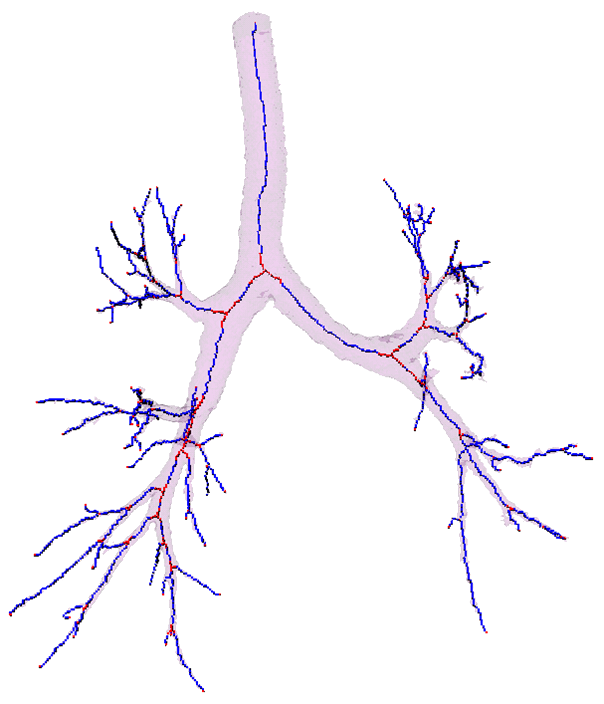
\includegraphics[height=2.5cm]{airways_segmentation.png}};
    \node (centerline_extraction)    [process, below of=lobes_segmentation, xshift=+2cm, yshift=-1cm]  {Centerline\\extraction};
    \node (surrogate_generation)     [process, right of=ct_acquisition, xshift=9.5cm]                  {Anatomical surrogate\\generation};
    \node (img_surrogate_generation) [image, above of=surrogate_generation, yshift=-.5cm]              {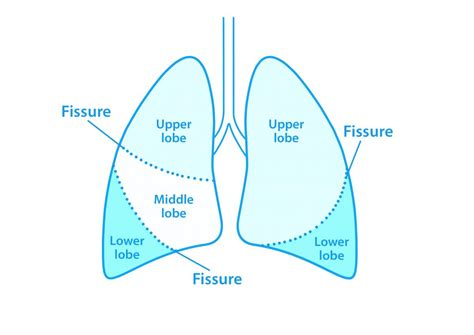
\includegraphics[width=3.5cm]{lobes_segmentation.jpg}};
    %% Julia & Mechanical Model
    \node (parameters_update)        [process, below of=ct_acquisition, yshift=-3cm]                   {Lungs parameters\\update};
    \node (model_instantiation)      [process, right of=parameters_update, xshift=1cm]                 {Mechanical model\\instantiation};
    \node (DAE_solution)             [process, right of=model_instantiation, xshift=1cm]               {DAE System\\solution};
    \node (simulations)              [startstop, right of=DAE_solution, xshift=+1cm]                   {Mechanical Simulations};

    % Arrows
    \draw [arrow] (ct_acquisition.east)                              -- ++(.5,0) coordinate(tmp)     |- (airways_segmentation.west);
    \draw [arrow] (airways_segmentation)                             -- (centerline_extraction);
    \draw [arrow] (centerline_extraction.east)                       -- ++(.5,0) coordinate(tmp1)    |- (surrogate_generation.west);
    \draw [arrow] (model_instantiation)                              -- (DAE_solution);
    \draw [arrow] (DAE_solution)                                     -- (simulations);
    \draw [arrow] (tmp)                                              |-   (lobes_segmentation.west);
    \draw [arrow] (lobes_segmentation)                               --   (tmp1|-lobes_segmentation) |- (surrogate_generation.west);
    \draw [dashed, thick, ->,>=stealth] (surrogate_generation.south) -- ++(0,-3.5)                   -| (parameters_update.north);
    \draw [arrow] (parameters_update)                                -- (model_instantiation);

    % Frame around a part of the flowchart
    \begin{pgfonlayer}{background}
      \node[rounded corners=3mm,
      draw=blue,
      thick, dashed,
      fit=(airways_segmentation)(centerline_extraction)(img_lobes_segmentation)(img_surrogate_generation),
      fill=cyan!5,
      inner sep=7pt,
      label={[anchor=north]below:\textsc{\textcolor{blue}{Chaste \& Morphometric model}}}] {};
    \end{pgfonlayer}
    \begin{pgfonlayer}{background}
      \node[rounded corners=3mm,
      draw=red,
      thick, dashed,
      fit=(parameters_update)(model_instantiation)(DAE_solution),
      fill=magenta!5,
      inner sep=7pt,
      label={[anchor=north]below:\textsc{\textcolor{red}{Julia Programming Language \& Mechanical model}}}] {};
    \end{pgfonlayer}
  \end{tikzpicture}
  \caption{Data pipeline.  The process begins with a
    \emph{patient-specific image} (i.e. CT) of a premature newborn.
    The extracted data, comprising \emph{two segmentations}, are then
    processed to obtain an anatomical surrogate of the airway tree.
    This is necessary due to scanner resolution not allowing for the
    discrimination and localization of small branches.  From the
    resulting morphometric model, the \emph{mechanical parameters} can
    be derived, which are essential for generating an accurate
    simulation model.  Finally, a numerical solver for differential
    equations provides the final output.}
    \label{fig:data_pipeline}
\end{figure}

%%% Local Variables:
%%% mode: LaTeX
%%% TeX-master: "../Thesis"
%%% End:

  % \begin{figure}[h!]
  \centering
  \scalebox{.75}{
    \begin{tikzpicture}[]
      % Nodes
      %% Chaste & Morphometric Model
      \node (ct_acquisition)           [startstop] {CT Acquisition};
      %%% Upper branch
      \node (lobes_segmentation)       [process, right of=ct_acquisition, xshift=8.25cm, yshift=+1cm]      {Lobes segmentation};
      \node (airways_segmentation)     [process, below of=lobes_segmentation, xshift=-2.5cm, yshift=-1cm]  {Airways segmentation};
      \node (centreline_extraction)    [process, below of=lobes_segmentation, xshift=+2.5cm, yshift=-1cm]  {Centreline extraction};
      \node (anatomical_generation)    [process, minimum width=5cm, text width=5cm, right of=ct_acquisition, xshift=16.5cm]                  {Algorithmic Generation of Distal Airway Centrelines};
      %% Julia & Mechanical Model
      \node (airways_model)            [startstop, below of=ct_acquisition, yshift=-5cm]               {Airways model};
      \node (acini_model)              [startstop, below of=airways_model, yshift=-1cm]                  {Acini model};
      \node (model_instantiation)      [process, below of=airways_segmentation, yshift=-5cm]                     {Mechanical model instantiation};
      \node (DAE_solution)             [process, below of=centreline_extraction, yshift=-5cm]               {DAE System solution};
      \node (tracheal_pressure)        [startstop, above of=DAE_solution, yshift=2.5cm]                      {Tracheal pressure waveform};
      \node (simulations)              [startstop, below of=anatomical_generation, yshift=-6cm]                   {Simulations results};
      \node (phi_length)               [startstop, minimum width=5cm, text width=4.5cm, above of=model_instantiation, yshift=2.5cm]                 {Diameters, length, father airway of each airway};
      
      
      % % Arrows
      \draw [arrow] (ct_acquisition.east)                              -- ++(1.5,0) coordinate(tmp)     |- (airways_segmentation.west);
      \draw [arrow] (airways_segmentation)                             -- (centreline_extraction);
      \draw [arrow] (centreline_extraction.east)                       -- ++(.5,0) coordinate(tmp1)    |- (anatomical_generation.west);
      \draw [arrow] (model_instantiation)                              -- (DAE_solution);
      \draw [arrow] (DAE_solution)                                     -- (simulations);
      \draw [arrow] (tmp)                                              |-   (lobes_segmentation.west);
      \draw [arrow] (lobes_segmentation)                               --   (tmp1|-lobes_segmentation) |- (anatomical_generation.west);
      \draw [arrow] (phi_length.south)  -- (model_instantiation.north);
      \draw [arrow] (acini_model.east) -- ++(1.5,0)  |- (model_instantiation.west);
      \draw [arrow] (tracheal_pressure.south) -- (DAE_solution.north);
      \draw [arrow] (airways_model.east) -- ++(1.5,0)  |- (model_instantiation.west);
      \draw [dashed, thick, ->,>=stealth] (12.5,-1.775) -- ++(0,-.50)                   -| (phi_length.north);

      
      % % Frame around a part of the flowchart
      \begin{pgfonlayer}{background}
        \node[rounded corners=3mm,
        draw=blue,
        thick, dashed,
        % fit=(airways_segmentation)(centreline_extraction)(img_lobes_segmentation)(img_anatomical_generation),
        fit=(airways_segmentation)(centreline_extraction)(lobes_segmentation)(anatomical_generation),
        fill=cyan!5,
        inner sep=7pt,
        label={[anchor=south]above:\textsc{\textcolor{blue}{Morphometric model}}}] {};
      \end{pgfonlayer}
      \begin{pgfonlayer}{background}
        \node[rounded corners=3mm,
        draw=red,
        thick, dashed,
        fit=(airways_model)(acini_model)(model_instantiation)(DAE_solution),
        fill=magenta!5,
        inner sep=7pt,
        label={[anchor=north]below:\textsc{\textcolor{red}{Mechanical model}}}] {};
      \end{pgfonlayer}
    \end{tikzpicture}
  }
  \caption{Data pipeline.  The process begins with a
    \emph{patient-specific image} (i.e. CT) of a premature newborn.
    The extracted data, comprising \emph{two segmentations}, are then
    processed to obtain an anatomical surrogate of the airway tree.
    This is necessary due to scanner resolution not allowing for the
    discrimination and localization of small branches.  From the
    resulting morphometric model, the \emph{mechanical parameters} can
    be derived, which are essential for generating an accurate
    simulation model.  Finally, a numerical solver for differential
    equations provides the final output.}
  \label{fig:data_pipeline}
\end{figure}

%%% Local Variables:
%%% mode: LaTeX
%%% TeX-master: "../Thesis"
%%% End:

  \caption{Data pipeline.  The process begins with a
    \emph{patient-specific image} (i.e. CT) of a premature newborn.
    The extracted data, comprising \emph{two segmentations}, are then
    processed to obtain an anatomical surrogate of the airway tree.
    This is necessary because scanner resolution does not allow for the
    discrimination and localization of small branches.  From the
    resulting morphometric model, the \emph{mechanical parameters} can
    be derived, which are essential for generating an accurate
    simulation model.  Finally, a numerical solver for differential
    equations provides the final output.}
  \label{fig:data_pipeline}
\end{figure}
  
%   2.2. Morphometric model
\subsection{Anatomical Model}
\label{subsec:airway_development}
% Per Chiara: Inserisco definizione di modello morfometrico?
Morphology generation process is required as it is not possible to
obtain high generations (aka small airways) using standard
high-resolution CT\cite{bordas2015}.

There are different open-source platforms available for generating
adult morphometric models.  In particular:

\begin{enumerate}
\item AVATree (Windows-only)
\item Chaste (cross-platform) library
\end{enumerate}

Due to problems related to «AVATree» source code compilation for
Windows with «Visual Studio», Chaste library is selected for this
project.

Chaste is a C++ open-source (BSD licensed) library developed by Oxford
University.  It has multiple use cases across various biomedical
fields, with an emphasis on cardiac electrophysiology and cancer
development\cite{mirams2013}.  It can be integrated into a C++ program
or used via «User Project» (i.e. \texttt{ctest}).  Specifically, the
``AirwayGenerationTutorial'' is considered as a first code base and
properly adapted to match newborn
parameters\cite{airwaygeneration2024}.

The required input consists of two pieces of information:
\begin{itemize}
\item A \emph{mesh of centreline points}.  This mesh is provided in
  TetGen format, comprising ``airways.node'' and ``airways.edge''
  files. The first file lists centreline point coordinates,
  respective sampled airways radius, and a boolean value to indicate if
  the point is generative. The second one contains all the connections
  between pairs of points.
\item Four (or five) \emph{lobes segmentations} in STL format.  These
  segmentations are necessary as they physically impose a limit on the
  growth algorithm.
\end{itemize}

\subsubsection{CT Image Processing: Lung Segmentation, Centreline and
  Radii Extraction}
\label{subsubsec:ct_centreline_radii_extraction}
% todo: Devo chiedere bene a Francesca come sono stati estratti i
% raggi.

«3D Slicer» is an open-source software used for CT image processing.
Two extensions are installed:

\begin{description}
\item «\emph{Chest\_imaging\_platform}»: This extension enables
  semi-automatic segmentation of major airways from a single fiducial
  point.  It can also extract adult lobes using three fiducial points
  per lung fissure. However, in our case, the fissures are not
  visible, necessitating manual intervention.
\item «\emph{SlicerVMTK}»: This extension is used for extracting
  centreline points.
\end{description}

\subsubsection{Algorithmic Generation of the Distal Airway Centreline}
\label{subsubsec:statistical_generation}

The Chaste User Project reads the input files
(see \cref{subsec:airway_development}), and begins growing the
anatomical surrogate from the points labeled as «generative».  The
algorithm operating under the hood is a modified version of the one
described in \cite{tawhai2000,bordas2015}.  The generated output is
available in various formats:

\begin{itemize}
\item VTU: Unstructured Grid (base64 encoded) format used by VTK
  library.  It can be displayed by ParaView, an open-source viewer.
\item node and edge: TetGen format.  Such files are better suited for
  further processing.
\end{itemize}

% bordas2015 parla anche di come vengono generate le vie aeree e come
% vengono assegnati i diametri.

% AGGIUNTA MODIFICA, COMPLETARE
% prima. -> SPOSTO LA FRASE IN SOTTOSEZIONE PARENTE.
This process is required as it is not possible to obtain high
generations (aka small airways) using standard high-resolution
CT\cite{bordas2015}.

The algorithm is based on a modified version of \textcite{tawhai2000}.
% {1} va spiegato qui, poi descriviamo l'algoritmo
A uniform grid of seed points is created within each segmented lobar
surface. Seed points approximately correspond to terminal bronchioles.
The spacing of the seed point grid is set so that the mean volume around
each of such points corresponds to the acinar volume (for adults being
$187\text{mm}^3$, for 5-weeks old newborns $5.3\text{mm}^3$).
% AGGIUNTA MODIFICA, COMPLETARE
% -> AGGIUNTO VALORE PER NEONATO 5W (da dove è stato recuperato?)

The starting points of the algorithm are the distal ends of the
segmented airway centrelines.  These points are referred to as growth
apices.

An \emph{adaptive threshold} on the distance between the seed points
and growth apices is required to prevent spurious long airways from being
generated in the last few generations.  \Cref{eq:airway_threshold}
describes such threshold:

\begin{equation}
  T = \max(V_{\text{b}} - n\cdot D_{\text{l}}, 5\text{mm})
  \label{eq:airway_threshold}
\end{equation}

Where:
\begin{description}
\item $V_{\text{b}}$ is the diagonal size of the bounding box of the lobe being
  generated into
\item $D_{\text{l}} (= {V_{\text{b}}/{N}})$ is the distance limit.
\item $N$ is the maximum number of generations.
\item $n$ is the current generation number.
\end{description}

With these definitions, the \textbf{growing algorithm} is described as
such:

\begin{enumerate}
\item \emph{Each seed point is associated with the closest growth apex
    within its lobe}.  The seed point having a distance to a
  growth apex greater than the aforementioned adaptive threshold is
  not associated with that distal end.  If all distal ends are further
  than the threshold from the seed point, the seed point remains
  unlabeled.
\item \emph{Calculation of the centroid of points assigned to each
    distal branch.}
\item \emph{The plane defined by the centroid and the parent branch is
    used to split the points into two unequal sets.}
\item \emph{Centroids of each of the new point sets are calculated.}
\item \emph{For each set of points a new airway is generated} starting
  at the distal end and extending 40\% of the distance towards the
  centroid of the point set.  This value is arbitrarily chosen for adults but kept for
  newborns.  It must be optimized in future developments.
\item \emph{Generated branches are checked to determine whether it is
    terminal}.  Branches whose length is less than $2\text{mm}$ (for
  adults, to be changed with $.12\text{mm}$ for newborns) are
  considered terminal.  Also, branches whose point set contains just a
  single point are considered terminal points.  For all
  terminal branches, their associated seed point is discarded from the
  global set.
\item \emph{Iterate} until no seed point is available.
\end{enumerate}

% DA DOVE VIENE FUORI .12 MM?
% sarebbe interessante capire come cambiare quel 2mm.

\textbf{Diameters} are computed by means of \cref{eq:lumen_diameter}.

\begin{equation}
  \log D(x) = (x - N)\log(R_{\text{d}} H) + \log(D_{\text{N}})
  \label{eq:lumen_diameter}
\end{equation}

Where:
\begin{description}
\item $D$ is the airway diameter.
\item $x$ is the current Horsfield order.
\item $N$ is the maximum Horsfield order.
\item $D_{\text{N}}$ is the maximum diameter.
\item $R_{\text{d}} H$ is the anti-log of the slope of airway diameter
  plotted against Horsfield order and is set to 1.15 for adults, 1.33
  for 5w newborns\cite[][Tab. 2]{horsfield1987}.  This parameter in
  the code is named ``DiameterRatio''.
\end{description}
  
\subsection{Mechanical Model}
\label{subsec:simulator_development}

In order to perform simulation it is required to use an efficient
differential equation solver.  «\texttt{DifferentialEquations.jl}»
wraps all available solvers (even C and FORTRAN ones) and it is very
efficient \cite{diffeqdocs2024,rackauckas2017}.

Julia is a free, open-source (MIT licensed), fast, scientific and
numerical computing-oriented programming language.  Its computational
efficiency is comparable to statically typed languages like C
or FORTRAN.  Moreover, its high-level code expressiveness rivals that of
languages like Python, R, and MATLAB\cite{juliadocs2024}.

Two key features, inspired by the \emph{Lisp Language}, are
highlighted here.

\begin{description}
\item \emph{Metaprogramming}: Code is treated as any other Julia data
  structure and, thus can be dynamically generated and manipulated at
  runtime.
\item \emph{Macros}: They help instantiate the generated code in the
  body of a program.
\end{description}

Their importance is closely tied to the concept of Domain-Specific
Languages (aka DSLs).  These dialects are composed of abstractions
that can be properly exploited to solve particular problems
(e.g. modeling complex systems, solving differential equations).

Julia REPL has a built-in package manager (i.e. «\texttt{Pkg.jl}»)
used for managing project dependencies and ensuring the
\emph{repeatability} of computational setups.  This is achieved by
saving the required package names and commits into `Project.toml' and
`Manifest.toml' files.

\subsubsection{Programming Language --- Model Designing \& Instantiating}
\label{subsubsec:modelingtoolkit}

«\texttt{ModelingToolkit.jl}» encompasses all the tools necessary for
model design.  This Julia package is equation-driven, requiring each
system to be described by Differential-Algebraic Equations (i.e. DAEs)
for subsequent solving\cite{ma2021}. Its built-in DSL optimizes every
stage of modeling, from prototyping components to instantiating the
complete system.

An acausal paradigm can be adopted, allowing users to reason in terms
of \emph{components}\cite{mtkdocs2024}. This modularity facilitates
system extensibility compared to the causal approach, where the entire
system of Differential-Algebraic Equations must be considered and
manually simplified\cite{ma2024}.

In particular, the usage of \jlinl{@mtkmodel} macro enables
hierarchical generation of building blocks recurring in the
highest-order model (i.e. «Lungs»).  Here is how information is
structured within \jlinl{@mtkmodel} macro.

\begin{jllisting}[label=@mtkmodel, caption={\jlinl{@mtkmodel}: a macro for systems prototyping.}]
  @mtkmodel <name_of_model> begin
      @parameters begin
          # (Optional) Some constant (e.g. Resistance, Capacitance) ...
      end
      @components begin
          # (Optional) Some dependency system (e.g. Resistor, Capacitor) ...
      end
      @variables begin
          # (Optional) Internal variables ...
      end
      @equations begin
          # Differential Algebraic Equations describing the model's behavior.
      end
      @continuous_events begin
          # (Optional) Some callback function ...
      end
  end
\end{jllisting}

Replicating the behavior of electrical components using this language
is straightforward, once you are familiar with the syntax and
understand the Differential-Algebraic Equations that represent their
characteristics.  Each generated system can then be composed into more
complex ones, using the internal \jlinl{@components} macro, thereby
implementing the hierarchical structure mentioned earlier.

After describing the highest-order system, the Julia compiler requires its
instantiation before any simulation can be performed.  This is
accomplished using \jlinl{@mtkbuild} macro, which minimizes the number
of equations that need to be solved.

Code modularity is directly reflected in the electrical equivalent
circuit.  Specifically, by encapsulating systems with the internal
\jlinl{@components} macro, it becomes possible to generate models of
increasing complexity.  This approach enables a clear separation
between components that belong to different hierarchical levels and
facilitates compartmentalization during the model design phase.

\vspace{.5em}

{\normalsize\textbf{Callbacks' Role in State Variables
      Discontinuity Handling}} Not all characteristics of electrical
components can be defined solely by DAEs.  Voltages or currents may
suddenly change, triggered by a circuit event.  In such cases,
\emph{continuous callback functions} can be employed to appropriately
alter the value of state variables.  These callbacks consist of two
functions:
\begin{itemize}
\item \texttt{condition}: Specifies the event to be tested.
\item \texttt{affect}: Defines how the state variable(s) should be
  changed.
\end{itemize}

The component-based approach allows for the definition of callbacks
directly within the (sub)system being modeled.

% Example of usage?

\subsubsection{Airways and Acini Models}
\label{subsubsec:blocks_description}


% 1. È necessario indicare la notazione utilizzata nelle formule?
% 2. Su cosa devo concentrarmi nella descrizione? Devo mostrare
% codice?

The following blocks are listed in a bottom-up order (from lowest to
highest).

\begin{enumerate}
\item \textbf{Mathematical and Electrical Components}.  The simplest
  blocks are derived from the standard library of components (aka
  «\texttt{ModelingToolkitStandardLibrary.jl}»), while integral-dependent
  ones rely on a modified mathematical block to manage both current
  integration and its timing correctly.  Their behavior varies based
  on the neonatal pulmonary fluid interface.
  \begin{description}
  \item \emph{Current Integrator}: it computes the current integral
    and manages integration timing through a Callback function
    (see the former Callbacks Section).
  \item \emph{Current Integral-Dependent Inductor}: It takes the
    current integral value from the Current Integrator and computes the
    inductance value according to this formula
    $L(t) = L_{\text{a}} + L_{\text{b}}\cdot \left(1 - \dfrac{\int
        {i(t) dt}}{V_{\text{FRC}}}\right)$, where $L_{\text{a}}$ is
    the inductance when air-filled, $L_{\text{b}}$ is the difference
    between liquid and air inductances, $V_{\text{FRC}}$ is the volume
    at FRC (i.e., Functional Residual Capacity).
  \item \emph{Current Integral-Dependent Resistor}: It takes the
    current integral value from the Current Integrator and computes the
    resistance value according to this formula
    $R(t) = R_{\text{a}} + R_{\text{b}}\cdot \left(1 - \dfrac{\int
        {i(t) dt}}{V_{\text{FRC}}}\right)$, where $R_{\text{a}}$ is
    the resistance when air-filled, $R_{\text{b}}$ is the difference
    between liquid and air resistances, $V_{\text{FRC}}$ is the volume
    at FRC.
  \item \emph{Diode}: It is modeled as a voltage generator whose
    activation state is dependent on the fill-up states of the
    previous and the current module ($\text{trigger}_{\text{in}}$ and
    $\text{trigger}_{\text{out}}$, respectively). Its behavior is
    summarized by the following formula:
    $\Delta V = \text{trigger}_{\text{in}} \cdot (1 -
    \text{trigger}_{\text{out}}) \cdot V_{\text{in,th}}$, where
    $\Delta V$ is the voltage drop across the component and
    $V_{\text{in,th}}$ is the diode voltage threshold. This is a
    custom component and it does not come as part of the standard
    library.
  \item \emph{Inductor}: Constant component.
  \item \emph{Resistor}: Constant component.
  \end{description}
\item \textbf{Modules}.  Obtained by connecting the aforementioned
  components together into functional models representing a
  physiological structure.
  \begin{description}
  \item
    \emph{Acinus} % Copiare didascalia (da trovare prima).
  \item \emph{Airway}.  It has a similar behavior in comparison to a
    transmission line.
  \end{description}
\item \textbf{Lungs}.  They represent the highest-order model because they are a combination of
  acini and airways.
\end{enumerate}

% Equivalent circuits for airways and acinus.
\begin{figure}[H]\centering
  \begin{circuitikz}[]
    % Circuit
    %% Main branch

    %%% Input Node
    \draw (1.5,0)
    node[ocirc] (circuit_IN) {}
    to[short, i=$i_{\text{in}}$, -*] ++(1.5,0) coordinate(D_SW_IN)
    ;
    
    %%% Diode // Switch branch
    \draw (D_SW_IN)
    to[short] ++(0,.5)
    to[diode, v^<=$V_{\text{in,th}}$, color=bluePoli] ++(2,0) coordinate(D_SW_OUT)
    to[short, -*] (D_SW_IN-|D_SW_OUT)
    ;
    \draw (D_SW_IN)
    to[short] ++(0,-.5)
    to[switch, color=bluePoli, a_=$\left(V_{\text{in}}\geq V_{\text{in,th}}\right) \lor \left(V_{\text{in}} \text{ = } 0\right)$] ++(2,0)
    to[short] (D_SW_IN-|D_SW_OUT)
    ;

    %% Main branch
    \draw (D_SW_IN-|D_SW_OUT)
    to[short] ++(.5,0)
    to[variable resistor, color=bluePoli, l=$R_{\text{tube}} / 2$] ++(2,0)
    to[variable inductor, color=bluePoli, l=$I_{\text{tube}} / 2$] ++(2,0) coordinate (C_g_IN)
    to[short] ++(1.5,0) coordinate (SW_IN)
    to[variable resistor, color=bluePoli, l=$R_{\text{tube}} / 2$] ++(2,0)
    to[variable inductor, color=bluePoli, l=$I_{\text{tube}} / 2$] ++(2,0)
    to[short, i=$i_{\text{out}}$] ++(1,0)
    node[ocirc] (circuit_OUT) {}
    ;

    %%% C_g branch
    \draw (C_g_IN)
    to[C=$C_{\text{g}}$, *-] ++(0,-3.5)
    node[ground]{} ++(0,0)
    ;

    %%% Sw branch
    \draw (SW_IN)
    to[L=$I_{\text{sw}}$, *-] ++(0,-1.5)
    to[R=$R_{\text{sw}}$] ++(0,-1)
    to[C=$C_{\text{sw}}$] ++(0,-1)
    node[ground]{} ++(0,0)
    ;
    
    %% Open circuit (input)
    \draw (circuit_IN)
    to[open, -o, v<=$V_{\text{in}}$] ++(0, -3.5)
    node[ground] {}
    ;
    %% Open circuit (output)
    \draw (circuit_OUT)
    to[open, -o, v^<=$V_{\text{out}}$] ++(0, -3.5)
    node[ground] {}
    ;

    % Nodes
    %% IN
    \draw  (circuit_IN.west)
    node[draw, anchor=east, color=white, fill=bluePoli!50] (node_IN) {IN}
    ;
    % \draw (node_IN.east) node[ocirc, right]{}
    % ;
    %% OUT
    \draw  (circuit_OUT.east)
    node[draw, anchor=west, color=white, fill=bluePoli!50] (node_OUT) {OUT}
    ;
  \end{circuitikz}
  \caption{Airway equivalent circuit.  In blue: all current integral-dependent components.}
  \label{fig:airway}

\end{figure}

%%% Local Variables:
%%% mode: LaTeX
%%% TeX-master: "../Thesis"
%%% End:

\begin{figure}[H]\centering
  \begin{circuitikz}[scale=.9]
    % Circuit
    %% Main branch

    %%% Input Node
    \draw (1.5,0)
    node[ocirc] (circuit_IN) {}
    to[short, i=$i_{\text{in}}$, -*] ++(1.5,0) coordinate(D_SW_IN)
    ;
    
    %%% Diode // Switch branch
    \draw (D_SW_IN)
    to[short] ++(0,.5)
    to[diode, v^<=$V_{\text{in,th}}$, color=bluePoli] ++(2,0) coordinate(D_SW_OUT)
    to[short, -*] (D_SW_IN-|D_SW_OUT)
    ;
    \draw (D_SW_IN)
    to[short] ++(0,-.5)
    to[switch, color=bluePoli, a_=$\left(V_{\text{in}}\geq V_{\text{in,th}}\right) \lor \left(V_{\text{in}} \text{ = } 0\right)$] ++(2,0)
    to[short] (D_SW_IN-|D_SW_OUT)
    ;

    %% Main branch
    \draw (D_SW_IN-|D_SW_OUT)
    % to[short] ++(.5,0)
    to[variable resistor, color=bluePoli, l=$R_{\text{tube}}$] ++(2.25,0)
    to[variable inductor, color=bluePoli, l=$I_{\text{tube}}$] ++(2.25,0) coordinate (circuit_OUT)
    % to[short] ++(.5,0)
    to[L=$I_{\text{t}}$] ++(2.25,0)
    to[R=$R_{\text{t}}$] ++(1.5,0)
    to[C=$C_{\text{t}}$] ++(1.5,0) coordinate (S_IN)
    % node[ocirc] (circuit_OUT) {}
    ;

    \draw (S_IN)
    to[short] ++(0,-.5)
    to[R, l_=$R_{\text{s}}$] ++(2,0)
    to[short] ++(0,.5)
    ;
    \draw (S_IN)
    to[short, *-] ++(0,.5)
    to[C=$C_{\text{s}}$] ++(2,0)
    to[short] ++(0,-.5)
    to[short, *-] ++(.5,0)
    node[ground]{} ++(0,0)
    ;

    %%% C_g branch
    \draw (circuit_OUT) node[draw, anchor=south, color=white, fill=bluePoli!50] {OUT}
    to[C=$C_{\text{g}}$, i=$i_{\text{out}}$, v<=$V_{\text{out}}$, *-] ++(0,-3.5)
    node[ground]{} ++(0,0)
    ;

    %% Open circuit (input)
    \draw (circuit_IN)
    to[open, -o, v<=$V_{\text{in}}$] ++(0, -3.5)
    node[ground] {}
    ;
    % %% Open circuit (output)
    % \draw (circuit_OUT)
    % {[red!60] to[open, -o, v^<=$V_{\text{out}}$] ++(0, -3.5)}
    % node[ground] {}
    % ;

    % Nodes
    %% IN
    \draw  (circuit_IN.west)
    node[draw, anchor=east, color=white, fill=bluePoli!50] (node_IN) {IN}
    ;
    % \draw (node_IN.east) node[ocirc, right]{}
    % ;
    %% OUT

  \end{circuitikz}
  \caption{Acinus equivalent circuit.  In blue: all current integral-dependent components.}
  \label{fig:acinus}

\end{figure}

%%% Local Variables:
%%% mode: LaTeX
%%% TeX-master: "../Thesis"
%%% End:



\subsubsection{Model Testing}
\label{subsubsec:model_testing}

Simulations are executed starting from a subtree (see
\cite{fig:subtree_development}), as the full circuit (comprising over
50k modules) requires more memory space than typically available on a
common laptop.

% \begin{figure}[H]
%   \centering
%   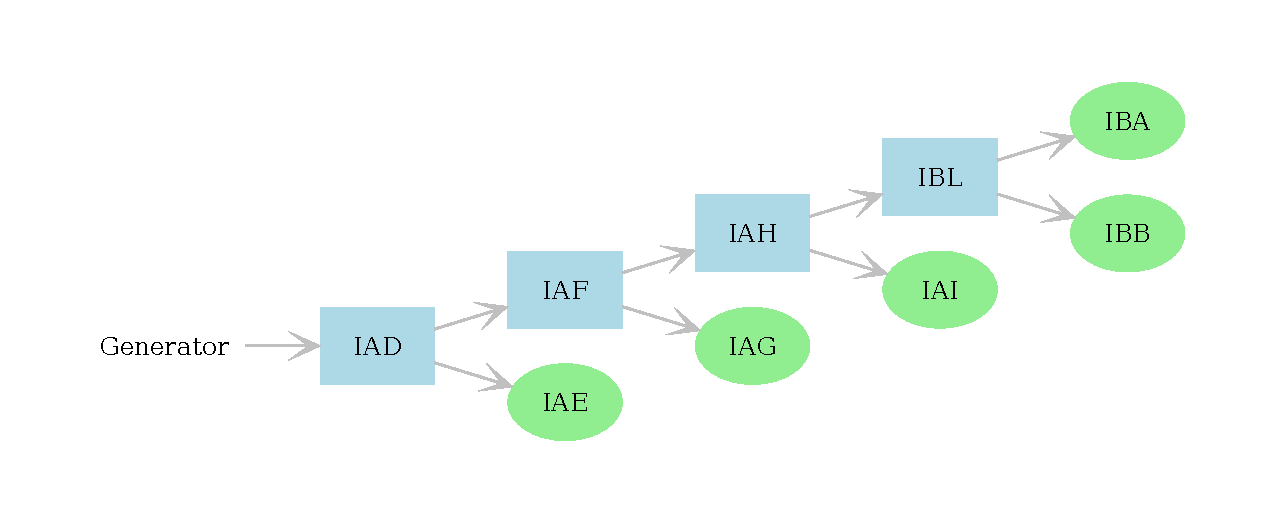
\includegraphics[scale=.7]{subtree.pdf}
%   \caption{The simulated subtree.  Airways are represented in light blue and acini in light green.}
%   \label{fig:subtree_development}
% \end{figure}

\begin{figure}[H]\centering
  \begin{tikzpicture}[node distance=2.3cm]
    \node (GEN) [rectangle, rounded corners, minimum width=1.5cm, minimum height=.75cm, draw=black, fill=green!25] {Generator};
    \node (IAD) [airway, right of=GEN, xshift=.25cm]              {\textsc{IAD}};
    \node (IAF) [airway, right of=IAD]                             {\textsc{IAF}};
    \node (IAH) [airway, right of=IAF]                             {\textsc{IAH}};
    \node (IBL) [airway, right of=IAH]                             {\textsc{IBL}};
    \node (IAE) [acinus, above of=IAD, xshift=.75cm]               {\textsc{IAE}};
    \node (IAG) [acinus, below of=IAF, xshift=.75cm]               {\textsc{IAG}};
    \node (IAI) [acinus, above of=IAH, xshift=.75cm]               {\textsc{IAI}};
    \node (IBA) [acinus, above of=IBL, xshift=.75cm]               {\textsc{IBA}};
    \node (IBB) [acinus, below of=IBL, xshift=.75cm]               {\textsc{IBB}};

    \draw [arrow1] (GEN) -- (IAD);
    \draw [arrow1] (IAD) -- (IAF);
    \draw [arrow1] (IAF) -- (IAH);
    \draw [arrow1] (IAH) -- (IBL);
    \draw [arrow1] (IAD) -- (IAE);
    \draw [arrow1] (IAF) -- (IAG);
    \draw [arrow1] (IAH) -- (IAI);
    \draw [arrow1] (IBL) -- (IBA);
    \draw [arrow1] (IBL) -- (IBB);
  \end{tikzpicture}
  \caption{The simulated subtree. Airways are represented in red,
    acini in blue.}
  \label{fig:subtree_development}
\end{figure}

%%% Local Variables:
%%% mode: LaTeX
%%% TeX-master: "../Thesis"
%%% End:



% In this project, Chaste has been relied upon to generate an anatomical
% surrogate for lungs in premature newborns.

%%% Local Variables:
%%% mode: LaTeX
%%% TeX-master: "../Thesis"
%%% End:
